\documentclass[autodetect-engine,dvipdfmx-if-dvi,ja=standard,a4j,jbase=10.5pt,twoside,twocolumn,magstyle=nomag*]{bxjsarticle}
% \documentclass[uplatex, dvipdfmx, a4j, 10ptj, twoside, twocolumn]{jsarticle}
% small japanese font size:     9pt, 10pt, 11pt, 12pt, 14pt, ... (please refer the document of jsclasses)
% word-like japanese font size: 10ptj 10.5ptj, 11ptj, 12ptj (or jbase=xxpt (without 'j') if error is occured)

\usepackage{ifptex,ifxetex,ifluatex}
\ifluatex
    \usepackage{bxcalcux}
    \ltjsetparameter{jacharrange={-2,-3}}
    \usepackage{luatexja-otf}
    \usepackage{bxbase}
\else\ifxetex
    % \usepackage{zxjatype}
    % \usepackage[macros]{zxotf}
    \XeTeXgenerateactualtext=1
    \usepackage{xltxtra}
    \usepackage{bxbase}
\else\ifuptex
    \usepackage{otf}
    \usepackage[prefernoncjk]{pxcjkcat}
    \cjkcategory{sym11,sym18,sym19}{cjk}
    \usepackage[utf8]{inputenc}
    \usepackage{pxbase}
\else\ifstrictptex
    \usepackage{otf}
    \usepackage[utf8]{inputenc}
    \usepackage{pxbase}
\fi\fi\fi\fi

\usepackage[LGR,T2A,T1]{fontenc}

\usepackage{graphicx}
% \usepackage[dvipdfmx]{graphicx}
\usepackage{grffile}

% paper layout setting
\setpagelayout{noheadfoot, left=18.0truemm, right=18.0truemm, top=29.0truemm, bottom=26.0truemm, columnsep=6.5truemm}
% \setpagelayout{noheadfoot, left=15.0truemm, right=5.0truemm, top=12.5truemm, bottom=12.5truemm, columnsep=5.0truemm}

% font setting
\usepackage{amsmath}
\usepackage{amssymb}
\usepackage{mathtools}
\usepackage{bm}
\usepackage{fix-cm}
\usepackage{newtxtext}
\usepackage[slantedGreek]{newtxmath}

% caption setting
\usepackage[font=bf,labelfont=bf,labelsep=quad]{caption}

% to balance the last page of the two-column article
% \usepackage[nospread, keeplastbox, nodebug]{flushend}

% title font style
\renewcommand{\headfont}{\bfseries}

% section setting (using titlesec, uelm package)
\renewcommand{\thesection}{\arabic{section}}
\renewcommand{\thesubsection}{\arabic{section}.\arabic{subsection}}

\usepackage[explicit]{titlesec}
\usepackage[normalem]{ulem}
\titleformat{name=\section}{\normalfont\headfont\normalsize\raggedright}{}{0pt}{\uline{\thesection.\quad#1}}
\titleformat{name=\section,numberless}{\normalfont\headfont\normalsize\raggedright}{}{0pt}{\uline{#1}}
% \titleformat{name=\section}{\normalfont\headfont\normalsize\raggedright}{}{0pt}{\thesection.\quad#1}
\titlespacing{name=\section}{0pt}{.5\Cvs plus .0\Cvs minus .3\Cvs}{.1\Cvs plus .0\Cvs minus .1\Cvs}
\titleformat{name=\subsection}{\normalfont\headfont\normalsize\raggedright}{}{0pt}{\thesubsection.\quad#1}
\titleformat{name=\subsection,numberless}{\normalfont\headfont\normalsize\raggedright}{}{0pt}{#1}
\titlespacing{name=\subsection}{0pt}{.3\Cvs plus .0\Cvs minus .2\Cvs}{.0\Cvs plus .0\Cvs minus .0\Cvs}

% \makeatletter
% \renewcommand{\section}{\@startsection{section}{1}{\z@}{.5\baselineskip}{.1\baselineskip}{\normalfont\normalsize\headfont\raggedright}}
% \renewcommand{\subsection}{\@startsection{subsection}{2}{\z@}{.3\baselineskip}{\z@}{\normalfont\normalsize\headfont\raggedright}}
% \makeatother

\usepackage{secdot}
\sectiondot{section}
\sectiondot{subsection}

% list (itemize, enumerate, description, ...)
\usepackage{enumitem}
\setlist[1]{parsep=.0\baselineskip,topsep=.2\baselineskip,itemsep=.1\baselineskip}
% \makeatletter
% \def\@listi{\leftmargin\leftmargini
%     \parsep \z@
%     \topsep .2\baselineskip
%     \itemsep .1\baselineskip \relax}
% \let\@listI\@listi
% \makeatother

% no page number
\pagestyle{empty}

% footnote
\usepackage[bottom,hang,stable]{footmisc}
\setlength{\footnotemargin}{0pt}

% float setting (figure, table)
\setlength\floatsep{2.0truemm}
\setlength\textfloatsep{2.0truemm}
\setlength\intextsep{1.0truemm}
\setlength\dblfloatsep{2.0truemm}
\setlength\dbltextfloatsep{2.0truemm}
\setlength\abovecaptionskip{0.5truemm}
\setlength\belowcaptionskip{0.5truemm}

% lineskip setting (body text, display-style equation)
\AtBeginDocument{%
    \narrowbaselines    % basic english lineskip (for article)
    % \widebaselines      % basic japanese lineskip
    %
    \setlength\abovedisplayskip{1.5truemm}    % equation setting
    \setlength\belowdisplayskip{1.5truemm}    % equation setting
}

% to suit ms-word template
\renewcommand{\baselinestretch}{0.9}


\makeatletter
%
% maketitle
% additional elements
\newcommand*{\etitle}[1]{\gdef\@etitle{#1}}
\newcommand*{\studentid}[1]{\gdef\@studentid{#1}}
\newcommand*{\laboarea}[1]{\gdef\@laboarea{#1}}
\newcommand*{\laboname}[1]{\gdef\@laboname{#1}}
%
% style definition
\def\@maketitle{%
\newpage%
\centering%
\let\footnote\thanks%
%
% title
{\fontsize{16.00truept}{16.00truept}\selectfont\headfont\@title\par}%
%
% english title
\ifx\@etitle\@undefined\else{\vspace{1truemm}{\fontsize{12truept}{12truept}\selectfont\headfont\@etitle\par}}\fi%
%
% name (option: student id)
\vspace{1truemm}%
\ifx\@studentid\@undefined\else{\fontsize{12truept}{12truept}\selectfont\headfont\@studentid\hspace{\Cwd}}\fi%
{\fontsize{12truept}{12truept}\selectfont\headfont\@author\par}%
%
% research area (\laboarea) and laboratory name (\laboname)
\ifx\@laboarea\@undefined%
    \ifx\@laboname\@undefined%
    \else\vspace{1truemm}{\fontsize{12truept}{12truept}\selectfont\headfont\@laboname\par}%
    \fi%
\else%
    \ifx\@laboname\@undefined\vspace{1truemm}{\fontsize{12truept}{12truept}\selectfont\headfont\@laboarea\par}%
    \else\vspace{1truemm}{\fontsize{12truept}{12truept}\selectfont\headfont\@laboarea\hspace{\Cwd}\@laboname\par}%
    \fi%
\fi%
%
%% old version (2 line) of research area (\laboarea) and laboratory name (\laboname)
%\ifx\@laboarea\@undefined\else{\vspace{1truemm}{\fontsize{10truept}{10truept}\selectfont\@laboarea\par}}\fi%
%\ifx\@laboname\@undefined\else{\vspace{1truemm}{\fontsize{10truept}{10truept}\selectfont\@laboname\par}}\fi%
%
%% date (error)
% \ifvoid\@date\else{\vspace{2truemm}{\fontsize{12truept}{12truept}\selectfont\@date\par}}\fi%
%
% abstract (no check)
\ifvoid\@abstractbox\else{\vspace{2truemm}{\centering{\fontsize{10truept}{10truept}\selectfont\box\@abstractbox\par}}}\fi%
\vspace{2truemm}%
}
%
%
% bibliography
\newcommand{\@bibsection}{\@startsection{section}{1}{\z@}{.5\baselineskip}{0.2\baselineskip}{\normalfont\fontsize{9truept}{11truept}\selectfont\headfont\raggedright}}
\setlength\bibindent{\Cwd}
\renewenvironment{thebibliography}[1]{%
    \global\let\presectionname\relax
    \global\let\postsectionname\relax
    \@bibsection*{\refname}\@mkboth{\refname}{\refname}%
    \list{\@biblabel{\@arabic\c@enumiv}}{%
        \settowidth\labelwidth{\@biblabel{#1}}%
        \leftmargin\labelwidth
        \advance\leftmargin\labelsep
        \setlength\itemsep{0.5truept plus 1.0truept minus 0.5truept}
        \@openbib@code
        \usecounter{enumiv}%
        \let\p@enumiv\@empty
        \renewcommand\theenumiv{\@arabic\c@enumiv}}%
    \fontsize{8truept}{9.5truept}\selectfont
    \sloppy
    \clubpenalty4000
    \@clubpenalty\clubpenalty
    \widowpenalty4000%
    \sfcode`\.\@m}
{\def\@noitemerr{\@latex@warning{Empty `thebibliography' environment}}\endlist}
%
\makeatother



%%%%%%%%%%%%%%%%%%%%%%%%%%%%%%%%%%%%%%%%%%%%%%%%%%%%%%%%%%%%%%%%%%%%%%%%%%%%%%%%


% title setting
\title{ストーリーコンテンツに対する日本語レビュー中の\\ネタバレ判別に関する研究}
\etitle{A Spoiler Detection Method for Japanese-written Reviews of Story Contents}
%\studentid{M16TB017}
\author{加守田 侑}
\laboarea{情報処理領域}
%\laboname{知識情報処理工学研究室}
\date{}


%%%%%%%%%%%%%%%%%%%%%%%%%%%%%%%%%%%%%%%%%%%%%%%%%%%%%%%%%%%%%%%%%%%%%%%%%%%%%%%%


% useful packages and settings
% table and array
\usepackage{array}
\usepackage{booktabs}   % \toprule, \midrule, \bottomrule in tabbler environment (with good spacing)
% \usepackage{tabularx}
\renewcommand{\arraystretch}{0.5}
\renewcommand{\doublerulesep}{1pt}

% caption
\usepackage{subcaption}
\captionsetup{compatibility=false}

% misc
\usepackage[nobreak]{cite}
% \usepackage[hyphens]{url}
% \usepackage{siunitx}
% \usepackage[nospread, keeplastbox, nodebug]{flushend} % to balance columns at last page

% in­tel­li­gent cross-ref­er­enc­ing
% usage:
% in middle of line: \cref{<label>}, \cref{<label1>,<label2>,...} 
% at head of line:   \Cref{<label>}, \Cref{<label1>,<label2>,...} 
\usepackage[capitalise,noabbrev]{cleveref}
% for japanese
\crefformat{chapter}{#2#1{}章#3}
\crefformat{section}{#2#1{}節#3}
\crefformat{subsection}{#2#1{}節#3}
\crefname{figure}{図}{図}
\crefname{table}{表}{表}
\crefname{equation}{式}{式}
\crefname{appendix}{付録}{付録}
\newcommand{\crefrangeconjunction}{--}
\newcommand{\crefpairconjunction}{,}
\newcommand{\crefmiddleconjunction}{,}
\newcommand{\creflastconjunction}{,}
\newcommand{\crefpairgroupconjunction}{,}
\newcommand{\crefmiddlegroupconjunction}{,}
\newcommand{\creflastgroupconjunction}{,}
% for english (only figure and table)
% \renewcommand{\figurename}{Fig.~}
% \renewcommand{\tablename}{Table~}
% \crefname{figure}{Fig.}{Figs.}
% \Crefname{figure}{Figure}{Figures}
% \crefname{table}{Table}{Tables}

% math font (integral, summation, product)
\ifptex
  \DeclareSymbolFont{cmlargesymbols}{OMX}{cmex}{m}{n}
  % \DeclareMathSymbol{\intop}{\mathop}{cmlargesymbols}{"5A}
  % \def\int{\intop\nolimits}
  % \DeclareMathSymbol{\ointop}{\mathop}{cmlargesymbols}{"49}
  % \def\oint{\ointop\nolimits}
  \DeclareMathSymbol{\sumop}{\mathop}{cmlargesymbols}{"58}
  \let\sum\sumop
  \DeclareMathSymbol{\prodop}{\mathop}{cmlargesymbols}{"59}
  \let\prod\prodop
\fi

% footnote style
\renewcommand{\thefootnote}{\arabic{footnote}}


%%%%%%%%%%%%%%%%%%%%%%%%%%%%%%%%%%%%%%%%%%%%%%%%%%%%%%%%%%%%%%%%%%%%%%%%%%%%%%%%


% document
\begin{document}

% title
\maketitle

%---------------
% はじめに
%---------------
\section{はじめに} \label{sec:intro}
オンラインショッピングサイトの多くには利用者が商品に関して自由に記述できる商品レビュー(以下,レビュー)が存在する.
レビューに記載されている他者の意見は商品購入の際に参考となる.
しかし,商品が漫画や小説などストーリーコンテンツの場合はネタバレがレビューに記載されている場合がある.
レビューに含まれるネタバレを読むことで,実際に商品を見た際の楽しみが減ってしまうので問題となる.

% ネタバレはレビュー全体に記載されている場合もあれば一部のみに記載されている場合もある.
本研究ではレビューを1文単位に分割し,ネタバレを含んだ文を判別することを目的とする.
日本語が持つ独特の文法や言い回しに対応するため,単語の分散表現とLong short-term memory (LSTM)\cite{lstm}を利用して判別を行う手法を提案する.

%---------------
% 関連研究
%---------------
\section{関連研究} \label{sec:kanren}
ストーリーコンテンツに関するネタバレを判別する研究として,田島ら\cite{tazima}はTwitterに投稿されたアニメ作品のネタバレツイートを判定する研究を行っている.
田島らは手動によるアニメ作品のジャンル分けを行い,各ツイートに含まれる特定の品詞の単語と文節の係り受け関係を特徴として,Support Vector Machine (SVM)で各ジャンルごとに学習および判別を行っている.
% また,田島らは判別するアニメ作品の番組情報が掲載されているサイトに記載されている人物を「主要人物」,「主要人物」以外で判別するアニメ作品のWikipedia記事に記載されている人物を「モブ」に分類し,人物名の置き換えを行うことで精度を向上させている.
% しかし,この手法では手動でアニメのジャンル分類を行っているため人手が必要となる.
しかし,この手法ではジャンルごとにネタバレか否かのタグ付けされたデータが必要となり汎用性がないと考えられる.

英語のレビューを対象にネタバレ(あらすじ)を判別する研究として,岩井らの研究\cite{iwai2}がある.
岩井らはAmazon.com上のストーリーコンテンツに関する英語のレビューを対象に1文単位であらすじの判別を行っている.
岩井らの提案手法は,あらすじとの相互情報量の大きい単語を主な特徴としてNaive Bayesで判別を行っている.
% あらすじ文が1523文,あらすじで無い文が3484文のデータセットに対して評価実験を行い,
% 結果としてNaive Bayesで最も精度の高いF値0.78を得ている.
岩井らは英語のレビューの場合,あらすじとの相互情報量の大きい単語として代名詞が多く含まれていることを述べている.
しかし日本語のレビューの場合,主語の省略が多いため代名詞による判別が難しいと考えられる.
また,あらすじとの相互情報量の大きい単語はタグ付けされた訓練データに含まれている単語しか考慮できず,未知語の多い文章の場合は判別の特徴として利用できないと考えられる.

%---------------
% 提案手法
%---------------
\section{提案手法}
本研究では,レビューの各文に含まれる単語をfastText\cite{fasttext}を用いて分散表現に変換し,LSTMによってネタバレを含む文の判定を行う.
またfastTextの訓練データとしてネタバレ判別実験に使用しないレビューを用いることで,ネタバレ判別実験の訓練データに依存しない分散表現を学習する手法を提案する.
提案手法の流れを\cref{fig:pmf}に示す.

\begin{figure}[t]
  \centering
  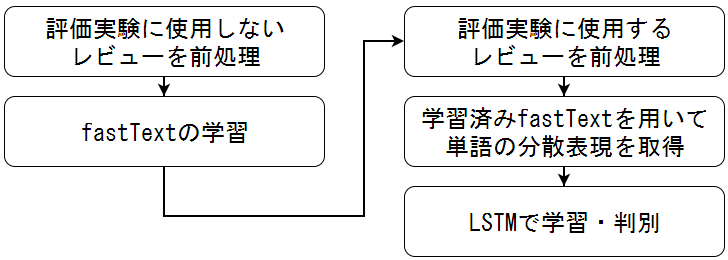
\includegraphics[width=1.0\linewidth, clip]{./figure/proposed_method_flow.png}
  \caption{提案手法の流れ}
  \label{fig:pmf}
\end{figure}

%---------------
% 前処理
%---------------
\subsection{前処理} \label{subsec:preprocessing}
まず,レビューを1文単位に分割するために,判別実験で使用するレビューを大まかに確認し,以下の10個の記号と改行コードで分割を行う.
\begin{center}
。?!? ! … ♪*\UI{2605}\UI{2606}
\end{center}

次に,各文を形態素解析器MeCab 0.996を用いて単語単位に分割する.
また,MeCabの辞書として新語辞書mecab-ipadic-NEologd v0.0.5を用いる.
単語単位に分割された文からネタバレを表す品詞と考えられる名詞・動詞・形容詞・形容動詞のみを抽出し,原型に直して判別に利用する.

%---------------
% 単語の分散表現取得
%---------------
\subsection{単語の分散表現取得}
単語の分散表現の取得にはfastTextを用いる.
単語の分散表現とは単語の意味を実数値のベクトルで表現したものである.
fastTextは同じ文脈に出現する単語は同じ意味を持つという分布仮説に基づいて学習を行う教師なし学習器である.
% 具体的に説明すると,ある文に含まれる単語を入力とし,その単語の前後に出現する単語を推測する.
% 推測した単語が元の文と同じになるように学習を行う教師なし学習器である.
fastTextは単語のサブワードの分散表現も同時に学習するため,未知語であっても学習済みのサブワードが含まれていれば分散表現を推測することができる.
本研究では単語の分散表現を100次元としてfastTextの学習を行った.

また,fastTextの訓練データにはネタバレ判別実験に使用しない商品のレビューを用いた.
これはネタバレ判別実験に使用するレビューに依存しない単語の分散表現を学習するためである.

%---------------
% LSTMによる学習・判別
%---------------
\subsection{LSTMによる学習・判別}
文を構成している単語の列を時系列データとしてとらえ,リカレントニューラルネットワークの一種であるLSTMをネタバレの判別器として利用する.
文に含まれる各単語の分散表現を順に入力し,学習および判別を行う.

使用するのは3層のニューラルネットワークである.
入力層が単語の分散表現に対応する100次元,中間層はLSTMのユニットを持つ50次元,出力層は2次元の全結合層とする.
入力層は0.2,中間層は0.5の割合でDropoutを行う.
出力層ではsoftmax関数を適用し,出力層の各次元をそれぞれネタバレである確率とネタバレでない確率としている.
また,各層の出力にはBatch Normalizationを適用している.

%---------------
% 評価実験
%---------------
\section{評価実験}
本研究では日本語のレビューデータセットとして,楽天株式会社が提供している楽天市場の商品に関するレビューデータセットを使用する.

%---------------
% データセット作成
%---------------
\subsection{データセット作成}
楽天市場の漫画カテゴリに含まれる商品の中で,5件以上のレビューが含まれる商品をランダムに100商品選択する.
選択した商品からそれぞれ5件のレビューをランダムに抽出する.
抽出した計500件のレビューを1文単位に分割し,各文がネタバレを含む文か否かを研究室の学生3名が各々の判断で判定した.
2人以上がネタバレと答えた文をネタバレを含む文とし,結果としてネタバレを含む文が182文,ネタバレを含まない文が1167文得られた.
これをネタバレ判別実験に使用するデータセットとする.
また,ネタバレ判別実験に使用しないレビューはfastTextの学習に利用する.

%---------------
% 学習・判別
%---------------
\subsection{学習・判別}
ネタバレ判別実験に使用するデータセットは小規模なので,10分割交差検定によって学習および判別を行う.
ニューラルネットワークは学習回数を200回,loss関数にクロスエントロピー,最適化アルゴリズムにAdadeltaを用いる.
判別実験に使用するデータセットは$1:6$の不均衡データセットであるため,loss関数計算時にクラスごとにデータ数に応じた重みを掛ける.

また,同じ商品レビューに対してネタバレの判別を行っている岩井らの手法を比較に用いる.
岩井らの手法は英語のデータセットでのみ評価しているため,今回使用した日本語のデータセットに適用して結果を比較する.
評価指標として適合率・再現率・F値を使用する.
\begin{itemize}
  \item $\text{適合率} = \frac{\text{正しく判別されたネタバレ文の数}}{\text{ネタバレと判別した文の数}}$
  \item $\text{再現率} = \frac{\text{正しく判別されたネタバレ文の数}}{\text{ネタバレ文の総数}}$
  \item $\text{F値} = \frac{2\ \times\ \text{適合率} \ \times\ \text{再現率}}{\text{適合率 + 再現率}}$
\end{itemize}

%---------------
% 結果
%---------------
\subsection{結果}
岩井らの手法と提案手法の実験結果を\cref{tab:kanren_exp}に示す.
\begin{table}[pt]
  \centering
  \caption{ネタバレ判別実験結果 \label{tab:kanren_exp}}
  \begin{tabular}{cccccc}
    \toprule %\hline
    手法 & 適合率 & 再現率 & F値 \\ \midrule % \hline
    \cite{iwai2}(英語・元論文) & 0.80 & 0.77 & 0.78 \\
    \cite{iwai2}(日本語) & 0.39 & 0.40 & 0.39 \\
    提案手法(日本語) & \textbf{0.47} & \textbf{0.67} & \textbf{0.55} \\
    \bottomrule % \hline
  \end{tabular}
\end{table}
英語のデータセットに対して行われた岩井らの手法の結果と比較すると日本語のデータセットでは岩井らの手法と提案手法の両方で大きく精度が下がっている.
原因の一つとして,判別実験用のデータセットのデータ数が少なかったことがあげられる.
また,日本語の場合は主語の省略や形態素解析時の誤りなど多岐にわたる要因により英語の場合に比べ精度が下がると考えられる.

次に日本語のデータセットの結果を比較すると,提案手法は全ての指標で岩井らの手法よりも精度が高くなっている.
これは2節で述べたように,岩井らの手法では代名詞の省略に対応できないため精度が低くなったと考えられる.
一方,提案手法は単語の分散表現を利用したことにより代名詞に頼らず,文に出現する単語の意味を用いて判別できたことが,精度が高くなった一因だと考えられる.
また,提案手法の結果では再現率が高くなっているため,より多くのネタバレを判別できていることがわかる.

%---------------
% まとめ
%---------------
\section{まとめ}
本研究では日本語のレビューデータに存在するネタバレが含まれる文の判別を,fastTextから得られた単語の分散表現とLSTMを用いて行う手法を提案した.
結果として,日本語のデータセットに対して関連研究の手法を適用した場合と比べ提案手法は精度が高くなり優位性が見られた.

今後の課題を述べる.
アンケート結果を確認すると,筆者の見解ではネタバレではないと思われる文がネタバレと判定されていた.
そのため,提案手法で作成された判別器をベースに利用者ごとにネタバレのタグ付けを行い学習させることで利用者に特化した判別器が作成され精度も向上すると考えられる.
また,レビューに含まれるネタバレ省く際,文脈が崩壊し,利用者がストレスを感じることになる.
そこで,文脈の崩壊度を定義し崩壊度が閾値以上の場合は,文脈がつながるように接続詞などで文章を修正する処理が必要となる.

%---------------
% 謝辞
%---------------
\section*{謝辞}
本研究ではデータセットとして,楽天株式会社が国立情報学研究所の協力により研究目的で提供している「楽天公開データ」を利用させていただきました.深く感謝いたします.

% bibliography
\begin{thebibliography}{9}

  %---------------------
  % Long short-term memory
  %---------------------
  \bibitem{lstm}
  F.~A. Gers, J.~A. Schmidhuber, and F.~A. Cummins, ``Learning to Forget: Continual Prediction with LSTM'', Neural Computation, vol.~12, no.~10, pp.~2451--2471, Oct.\ 2000.

  %---------------------
  % 関連研究
  %---------------------
  \bibitem{tazima}
  田島一樹, 中村聡史, ``Twitterにおけるアニメのネタバレツイート判定手法の提案'', 第8回データ光学と情報マネジメントに関するフォーラム(DEIM), 2016.

  \bibitem{iwai2}
  岩井秀成, 土方嘉徳, 西田正吾, ``レビューの文脈一貫性を用いたあらすじ文判定手法'', 情報処理学会論文誌・データベース, vol.~7, no.~2, pp.~11--23, Jun.\ 2014.

  %---------------------
  % fastText
  %---------------------
  \bibitem{fasttext}
  P. Bojanowski, E. Grave, A. Joulin, and T. Mikolov, ``Enriching Word Vectors with Subword Information'', Transactions of the Association of Computational Linguistics, vol.~5, pp.~135--146, 2017.

\end{thebibliography}

\end{document}